

\chapter{Conception}

\section{Diagramme de classe}
Le diagramme de classe permet de visualiser les principales entités de l'application et leurs relations.\\
Dans notre application, les entités principales incluent Utilisateur, Commande, Panier, Produit, Boisson, Ingredient, Supplement, ImageProduit, ProduitDansPanier, BoissonDansPanier, IngredientDansProduitDansPanier, SupplementDansProduitDansPanier, Categorie, Produit du jour.\\
Ces entités sont liées entre elles par des relations spécifiques, qui seront représentées sous forme de classes et d'associations.\\

Voici une explication des classes et de leurs relations dans notre modèle :
\begin{itemize}
    \item \textbf{AspNetUsers} : Un utilisateur dans le système \texttt{ASP.NET Identity}, représenté dans la table \texttt{AspNetUsers}, peut être un client ou un administrateur. Pour faire la distinction, il suffit d'examiner la table \texttt{AspNetRoles} et de vérifier si l'utilisateur est associé au rôle admin via une relation dans la table de jonction entre \texttt{AspNetUsers} et \texttt{AspNetRoles}.

    Le diagramme de classe Users peut être représenté de la manière suivante : \\
    \begin{figure}[H]
        \centering
        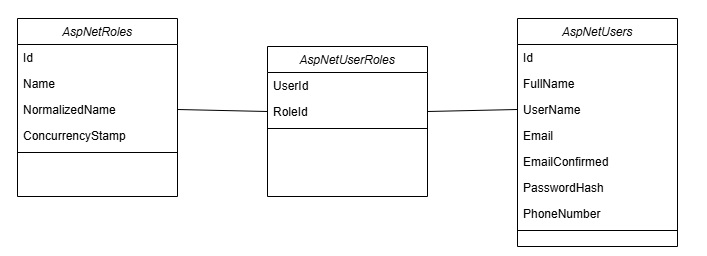
\includegraphics[width=0.8\columnwidth]{DiagClassUsers}
        \caption{Diagramme de classe - Identity User}
        \label{fig:class_users}
    \end{figure}
    
    \item \textbf{Product} : La table \texttt{Product} représente un article destiné à la consommation dans le restaurant.

    \item \textbf{Category} : La table \texttt{Category} permet de classer les produits en différentes catégories afin d'organiser efficacement le menu.

    \item \textbf{Ingredient} : La table \texttt{Ingredient} centralise les informations relatives aux ingrédients utilisés dans les produits. Chaque ingrédient est identifié par un nom. Cette table permet d'associer des ingrédients spécifiques à chaque produit via une relation avec la table \texttt{Product}.

    \item \textbf{Supplement} : La table \texttt{Supplement} contient les informations sur les suppléments associés aux produits. Chaque supplément est défini par un nom et un prix. Cette table facilite la gestion centralisée des suppléments et leur association aux produits via une relation avec la table \texttt{Product}.

    \item \textbf{Image} : La table \texttt{Image} stocke les informations relatives aux images des produits du restaurant. Chaque image peut représenter un plat ou un produit spécifique, afin d'améliorer la présentation visuelle du menu.

    \item \textbf{Drink} : La table \texttt{Drink} répertorie les boissons disponibles dans le restaurant. Elle contient des informations telles que le nom, le prix et d'autres caractéristiques pertinentes. Chaque boisson peut être ajoutée à un panier via la table \texttt{DrinkCart}, permettant ainsi au client de sélectionner une boisson en complément de sa commande.

    \item \textbf{ProductOfTheDay} : La table \texttt{ProductOfTheDay} met en avant un produit spécifique du menu chaque jour, comme une offre spéciale ou un plat du jour. Elle est liée à la table \texttt{Product} via un identifiant (\texttt{ProductId}).

    Le diagramme de classe reliée au gestion du stock peut être représenté de la manière suivante : \\
    \begin{figure}[H]
        \centering
        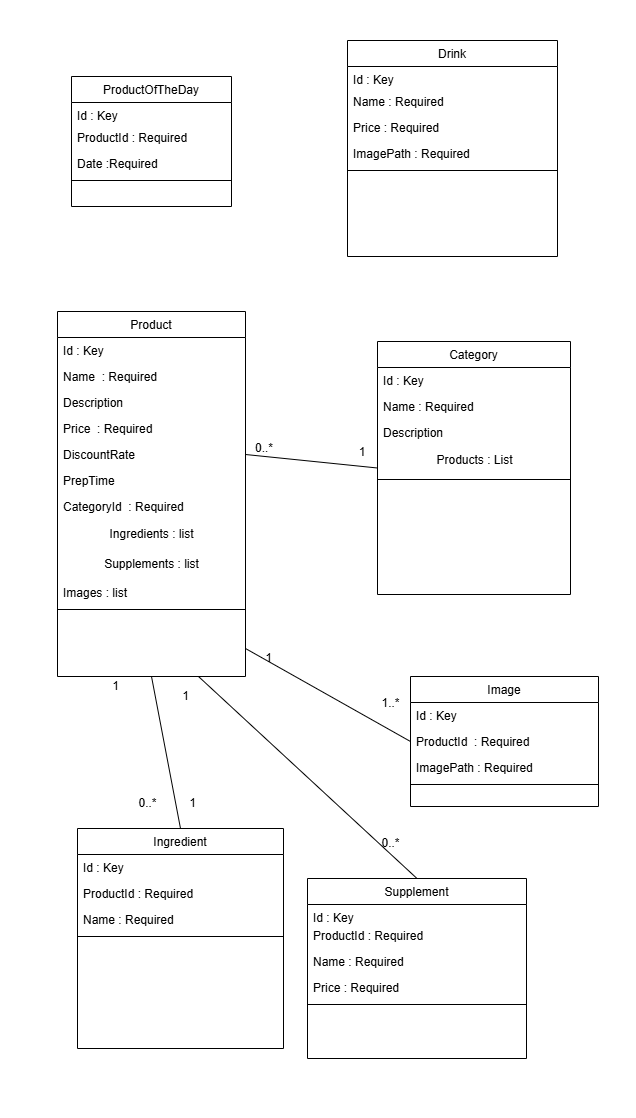
\includegraphics[width=0.8\columnwidth]{DiagClassAdmin}
        \caption{Diagramme de classe - Gestion du stock}
        \label{fig:class_admin}
    \end{figure}
    
    \item \textbf{Cart} : La table \texttt{Cart} représente le panier, qui regroupe l'ensemble des produits et boissons sélectionnés par un client avant la finalisation de la commande.

    \item \textbf{Order} : La table \texttt{Order} représente une commande passée par un client. Elle contient les informations essentielles telles que l'identifiant de la commande, le statut, la date, un message, et l'identifiant du panier associé.


    \item \textbf{ProductCart} : La table \texttt{ProductCart} est utilisée pour gérer les produits ajoutés au panier d'un client. Elle enregistre chaque produit, sa quantité ainsi que ses options supplémentaires (telles que \texttt{ProductCartIngredient} et \texttt{ProductCartSupplement}) lors de la commande. Cette table est liée à la table \texttt{Cart}, ce qui permet de suivre précisément les produits associés à chaque panier.

    \item \textbf{ProductCartIngredient} : La table \texttt{ProductCartIngredient} stocke les ingrédients ajoutés aux produits présents dans le panier.

    \item \textbf{ProductCartSupplement} : La table \texttt{ProductCartSupplement} stocke les suppléments ajoutés aux produits présents dans le panier.

    \item \textbf{DrinkCart} : La table \texttt{DrinkCart} gère la relation entre les boissons et les commandes dans le panier.
    
    Le diagramme de classe reliée au commande et panier peut être représenté de la manière suivante : \\
    \begin{figure}[H]
        \centering
        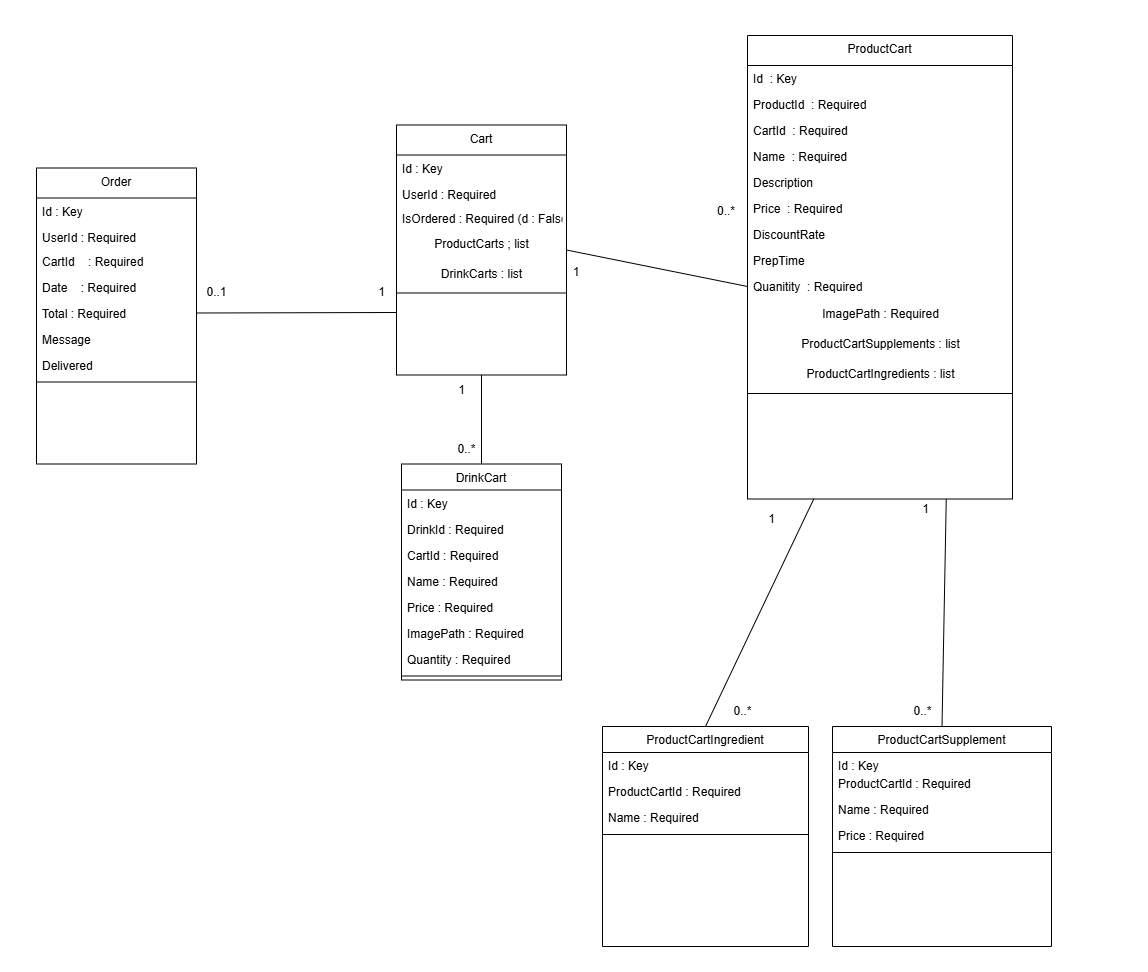
\includegraphics[width=0.8\columnwidth]{DiagClassCart}
        \caption{Diagramme de classe - commande et panier}
        \label{fig:class_cart}
    \end{figure}
    
\end{itemize}
\newpage

\section{Diagramme des cas d’utilisation}
Le diagramme des cas d'utilisation illustre les différentes interactions entre les utilisateurs et l'application, en distinguant les fonctionnalités accessibles à chaque type d'utilisateur. L'application est structurée en deux parties principales : Client et Administrateur.

\section*{Client}
Le diagramme de cas d'utilisation peut être représenté de la manière suivante : \\
\begin{figure}[H]
    \centering
    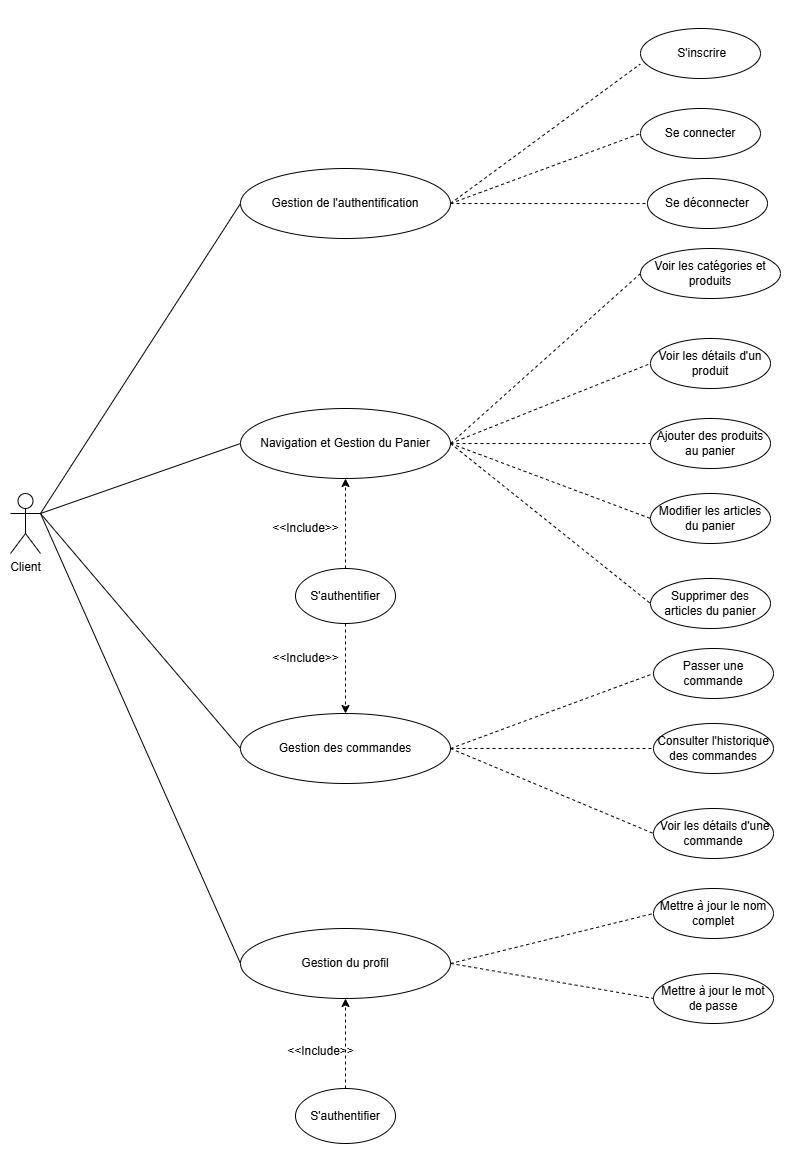
\includegraphics[width=0.7\columnwidth]{DiagUseCaseClient}
    \caption{Diagramme de cas d’utilisation - Client}
    \label{fig:usecase_client}
\end{figure}

\section*{Admin}
Le diagramme de cas d'utilisation peut être représenté de la manière suivante : \\
\begin{figure}[H]
    \centering
    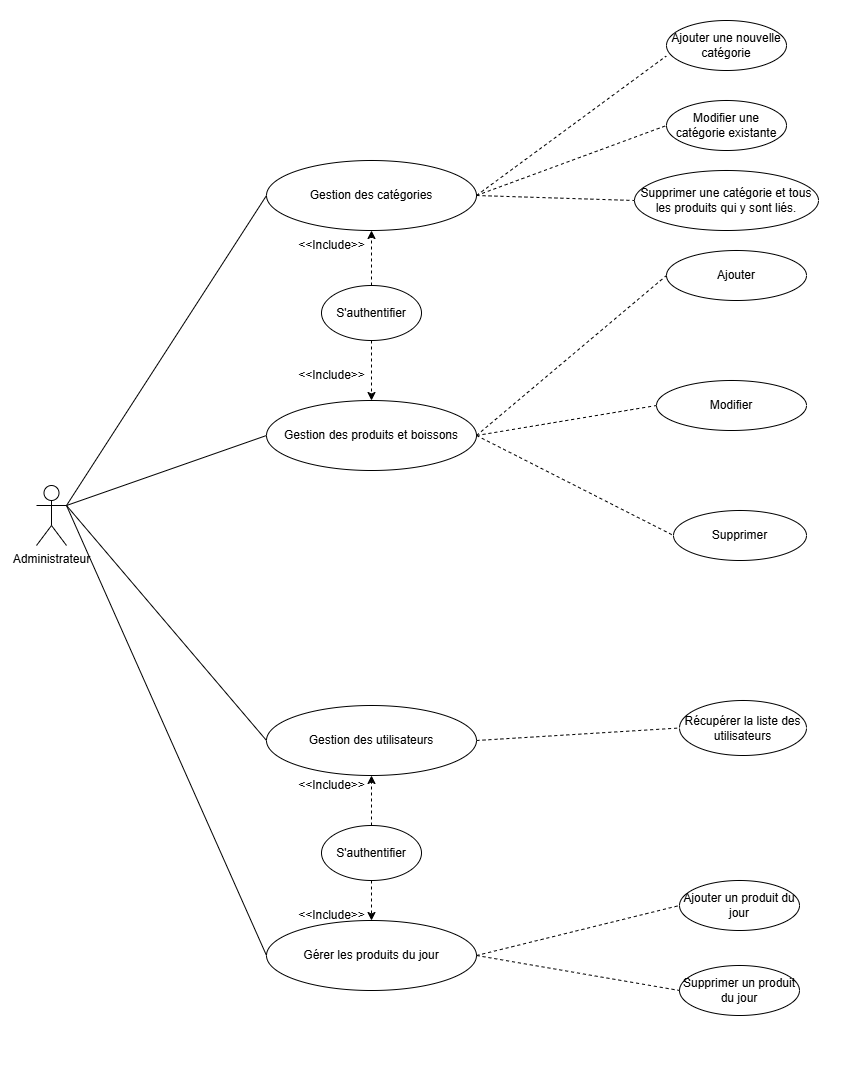
\includegraphics[width=0.8\columnwidth]{DiagUseCaseAdmin}
    \caption{Diagramme de cas d’utilisation - Admin}
    \label{fig:usecase_client}
\end{figure}

\section*{Conclusion}
Les diagrammes de classe et de cas d'utilisation sont essentiels pour modéliser la structure et le comportement de l'application. Ils aident à mieux comprendre les relations entre les entités et les actions possibles pour chaque type d'utilisateur, facilitant ainsi le développement et la maintenance de l'application.



\section{Diagrammes de Séquence}

Les diagrammes de séquence permettent de représenter le déroulement chronologique des interactions entre les utilisateurs (Client et Administrateur) et le système. Ils décrivent l’échange de messages entre les différents composants de l'application pour chaque fonctionnalité clé.

Pour notre application, trois diagrammes principaux sont présentés : l'Authentification, la creation d'un compte client et l'Ajout de produit au panier.

\section*{Authentification}
Le diagramme ci-dessous représente les interactions permettant à un utilisateur (Client ou Administrateur) de s'authentifier dans l'application :

\begin{figure}[H]
    \centering
    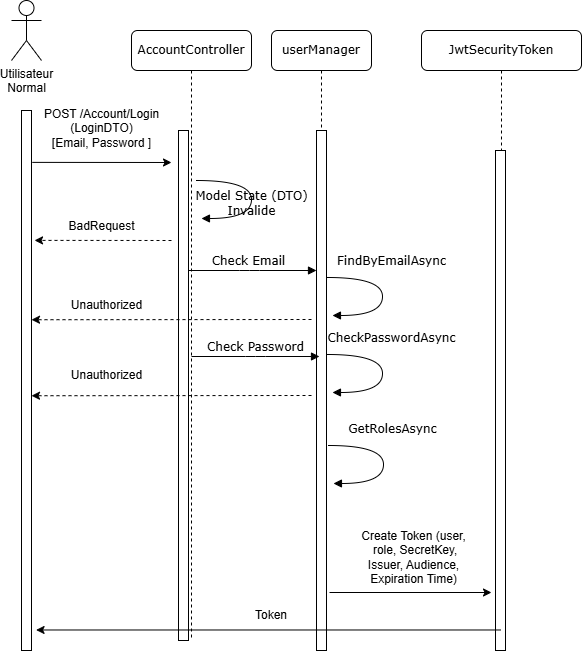
\includegraphics[width=0.5\columnwidth]{DiagSeqAuth}
    \caption{Diagramme de séquence - Authentification}
    \label{fig:seq_auth}
\end{figure}

\section*{Création du compte client}
Le diagramme ci-dessous représente les différentes étapes permettant à un client de créer un compte dans l'application :  
\begin{figure}[H]
    \centering
    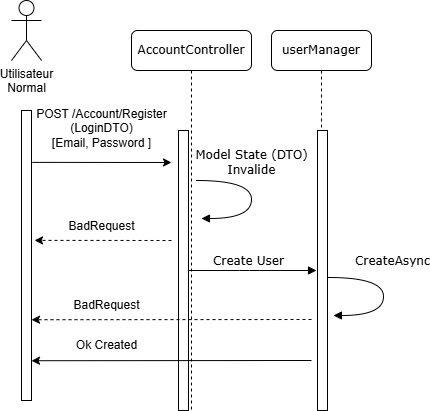
\includegraphics[width=0.5\columnwidth]{DiagSeqRegister}
    \caption{Diagramme de séquence - Création de compte client}
    \label{fig:seq_register}
\end{figure}

\section*{Ajout d'un produit au panier du client}
Le diagramme suivant illustre les interactions liées à l'ajout d'un produit dans le panier du client :  
\begin{figure}[H]
    \centering
    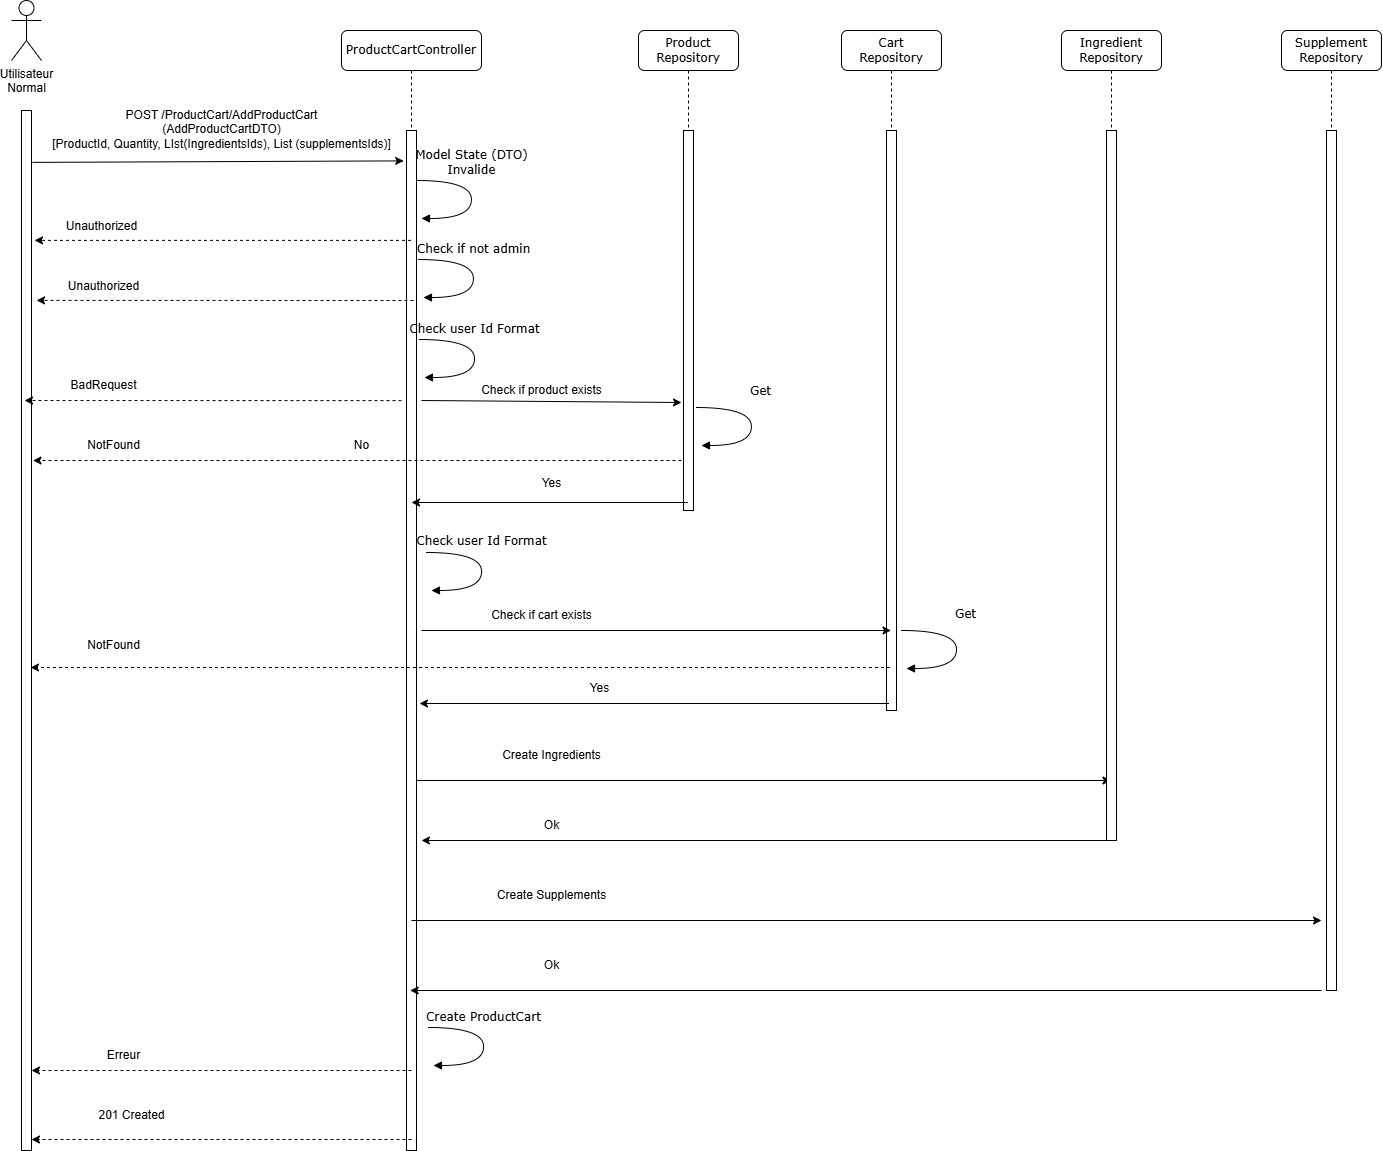
\includegraphics[width=0.8\columnwidth]{DiagSeqAddProductCart}
    \caption{Diagramme de séquence - Ajout d'un produit au panier}
    \label{fig:seq_addtocart}
\end{figure}


\section*{Conclusion}

Les diagrammes de séquence présentés illustrent les interactions clés entre les utilisateurs (Client et Administrateur) et le système. Le diagramme d'authentification montre le processus de connexion des utilisateurs. Celui de la création de compte client décrit l'enregistrement d'un nouvel utilisateur. Enfin, le diagramme d'ajout d'un produit au panier présente l'interaction du client avec le système pour ajouter des produits. Ces diagrammes permettent de visualiser le flux des interactions et la communication entre les différents composants de l'application.
